\section{Step Detection Algorithm}
The algorithm used to detect steps is described in this section. The terms not obvious are also described here:
\begin{description}
\item[Gait Speed] is the interval between two steps, and measuring it is useful, as it can be used to measure Risk for falling and as a shorthand for physical ability.
\item[Gait variability] is the standard deviation for gait speed over time. This is significant, because a large variability is correlated with increased risk for falling.
\end{description}
\subsection{Development and purpose of Algorithm}
As the group had little experience in sensor use and signal processing, a series of experiments were conducted to better understand which sensors provide useful information for step detection, and which patterns predicate steps. To this end, a simple app was developed to observe sensor input and store the raw data as a file, which then could be transferred to a computer. A set of Python scripts were written to plot  the data time series. Using Python, the group experimented with different step detection algorithms, and a computer-based prototype was developed. Finally, the algorithm was implemented in the Valens Step Detector app, modified to work with live data.

\subsection{Core Algorithm}\label{def:coreAlgorithm}
The current section will explain the algorithm used for step detection, formulated as an off-line algorithm. The following section will explain what changes were made to make the algorithm work for live data streams.

Experiments showed that the accelerometer consistently gave the most predicative feedback patterns for step detection\footnote{None of the android phones available to the group at the time had a working gyroscope. It is suspected that a gyroscope can replace or supplement the accelerometer for more precise step detection, but this should be tested empirically.}. Furthermore, it was found that the total acceleration was a better predicator of steps than acceleration along any of the single axes individually. To exploit this, a pre-processing step calculates the vector length in euclidean space of the raw acceleration vector.

Detecting steps based on a time series of acceleration vector lengths reduces to peak detection in the time series graph. The step detection algorithm is therefore essentially a generic algorithm for peak detection in noisy data. The noise in the data originates from noise in the sensor readings. To cope with the noise, the data is first smoothed using a moving average\footnote{That is, every data point has its value set to the average of itself and the k neighbors before and after it, where k is a constant referred to as the \emph{window size} of the smoothing.}. A larger value of k gives a smoother curve, but a too large value of k may flatten the graph too much.

Subsequently the program runs the main peak detection algorithm, which consists of the following steps:
\begin{description}

\item[Calculate peak strength] \hfill \\
Every data point in the time series has its \emph{peak strength} calculated. Informally, the peak strength of a data point is a measurement of how much that point is worthy of being considered a peak. A wide range of functions can map the raw vector lengths into a peak strength graph, but an additional desideratum of the peak strength function is that the output values should be normalized around 0. With the peak strength function used in the current implementation the peak strength of the point $x_i$ is calculated as $$\frac{\frac{(x_{i} - x_{i-1} + x_{i} - x_{i-1} + \ldots + x_{i} - x_{i-k})}{k} + \frac{(x_{i} - x_{i+1} + x_{i} - x_{i+1} + \ldots + x_{i} - x_{i+k})}{k}}{2},$$ where k is a constant referred to as the \emph{peak strength window}. 

\item [mean and standard deviation] \hfill \\
The mean, $\mu$, and standard deviation, $\sigma$, of all positive peak strength values are calculated. Sub-zero values are discarded.

\item[Search for potential peaks] \hfill \\
Every data point in the peak strength series is classified as either a potential peak or discarded. A data point i is classified as a potential peak if its peak strength value $x_i$ is positive and fulfils the following inequality: $x_i - \mu > k * \sigma$, where k is a constant, referred to as the \emph{std threshold}. The larger the value of k, the fewer data points are classified as peaks. This step thus functions as a high-pass filter, where the cut-off threshold is defined dynamically by $\mu$ and k.

\item[Remove close peaks] \hfill \\
If two data points that have been classified as potential peaks are very close to each other, it is likely that they both belong to the same peak in the actual data. To avoid peaks in the data from being classified multiple times, this step runs through the list of potential peaks, and for every pair of potential peaks it removes the least strong peak if they are closer than some constant k. In the current implementation, k is set to the same value as the peak strength window, following the approach taken in \cite{SimplePeakDetect}.

\end{description}

The data points that remain after the application of the algorithm are counted as steps.

\subsection{Application of the algorithm to live data}
The algorithm as stated above works on an off-line time series of data, and adapting it to work with live data requires some non-trivial decisions to be made, most of which will be explained and elaborated upon in this section. 

While it is possible to change the algorithm to run completely on-line, classifying every new vector length data point as either a step or not, thus reporting steps exactly as the happen, this approach is problematic. Firstly, as no data exists past the newest data point, only the previous data points can be used for smoothing and peak strength calculation. This can potentially reduce the precision of smoothing and peak strength calculation significantly. Therefore, a semi-live approach has been taken, in which a fixed number of data points are collected before step detection is performed. The collected data is then discarded, and the process start over again. However, some care needs to be taken to ensure that all the data is used, and no data points are used multiple times. The first and last $k$ (the smoothing window) data points cannot be used for step detection, because there is not sufficient data to smooth them properly. Likewise, the first and last $n$ (peak strength window) data points cannot have their peak strength calculated properly, and are not used for step detection. Because of this, the last $2n + 2k$ data points are retained when the collected data is discarded, as the last $n+k$ data points have only been used for smoothing and peak strength calculation, not for step detection, and the $n+k$ data points before that - which have already been used for step detection - are required for smoothing and peak strength calculation in the next batch of data.

Another issue when working with live data is how to calculate $\mu$ and $\sigma$. First of all, calculation of $\sigma$ requires the entire data series, but retaining the entire series of raw data in main memory is infeasible. Also, in a real life application long periods of inactivity will reduce $\mu$ to unnaturally low levels, potentially creating false positives during step detection. A better solution is to base calculation $\mu$ and $\sigma$ on actual movement data, so the values are adjusted to the relevant movement characteristics of the person. Based on these motivations, the app first requires the user to calibrate it by walking for 30 seconds. Values $\mu$ and $\sigma$ are thus calculated once based on the time series generated during calibration. 

\subsection{Constant values}
\label{constant_values}
The constants used by the algorithm play a significant role, and finding good values for these constants is crucial for the performance of the algorithm. However, there it is impossible to know a priori which values give the desired result, but it should be noted that some of the constants (particularly the window size constants) are related to the frequency at which sensor data is generated\footnote{That is, the faster the sensor data is generated, the wider the windows can be without increasing the risk for mixing information between separate peaks.}. Because of this, most constant values have been found by empirical studies during the prototyping step, so there might exist room for improvement, but thorough empirical studies or machine learning techniques may be required to uncover better values for the constants.

\subsection{Gait calculations}
To calculate the Gait variables, the step detections is used as base data. The step detection data is based on time in milliseconds since 1 January 1970 00:00:00 UTC/GMT (Unix epoch), usually referred to as a timestamp. This makes it easy to calculate mean times, intervals and standard deviation, which is the numbers we want for the two Gait parameters. To lower the fault rate in this data, periods of walking less than 10 seconds is discarded. This because of input from health experts saying that periods less than 10 seconds usually refers to inside walking, and is not suitable to do calculations with due to differences in indoor and outdoor walking Gait parameters.\\
The data is calculated by a calculation service inside the Content Provider and is scheduled to run once a day. The longer the time and the larger the amount of data, the more accurate calculations is able to be done, since the calculations is based on averages.

\subsection{Room for improvement}
\label{step_detector_improvements}
The current step detector is rather primitive, and has room for improvements in several areas. Testing has however shown the step detector to perform within acceptable limits, at least for a prototype-stage application. The effort required to produce significant improvements to the step detector was therefore not justifiable given the time limits of the project. However, step detector improvement appears to be a major concern if the application is to be developed further.

The following areas of improvement have been identified:
\begin{enumerate}
\item Because the phone is kept in a pocket, it is closer to one of the legs. This results in accelerometer output for movement in one foot being significantly higher than the other. Figure \ref{fig:FilipWalks} illustrates this phenomenon. A step detection algorithm that exploits this fact will necessarily be more precise than the current algorithm, which does not. However, it is hard to see exactly such how an algorithm can be devised.
\item Several different functions can be used for peak detection, and experimentation with different functions could possibly improve detector performance.
\item Constant values could be tweaked further (see section \ref{constant_values} on Constant Values)
\end{enumerate}

\begin{figure}[p]

\setlength\fboxsep{0pt}
\setlength\fboxrule{1pt}\noindent\makebox[\textwidth]{%
 \fbox{
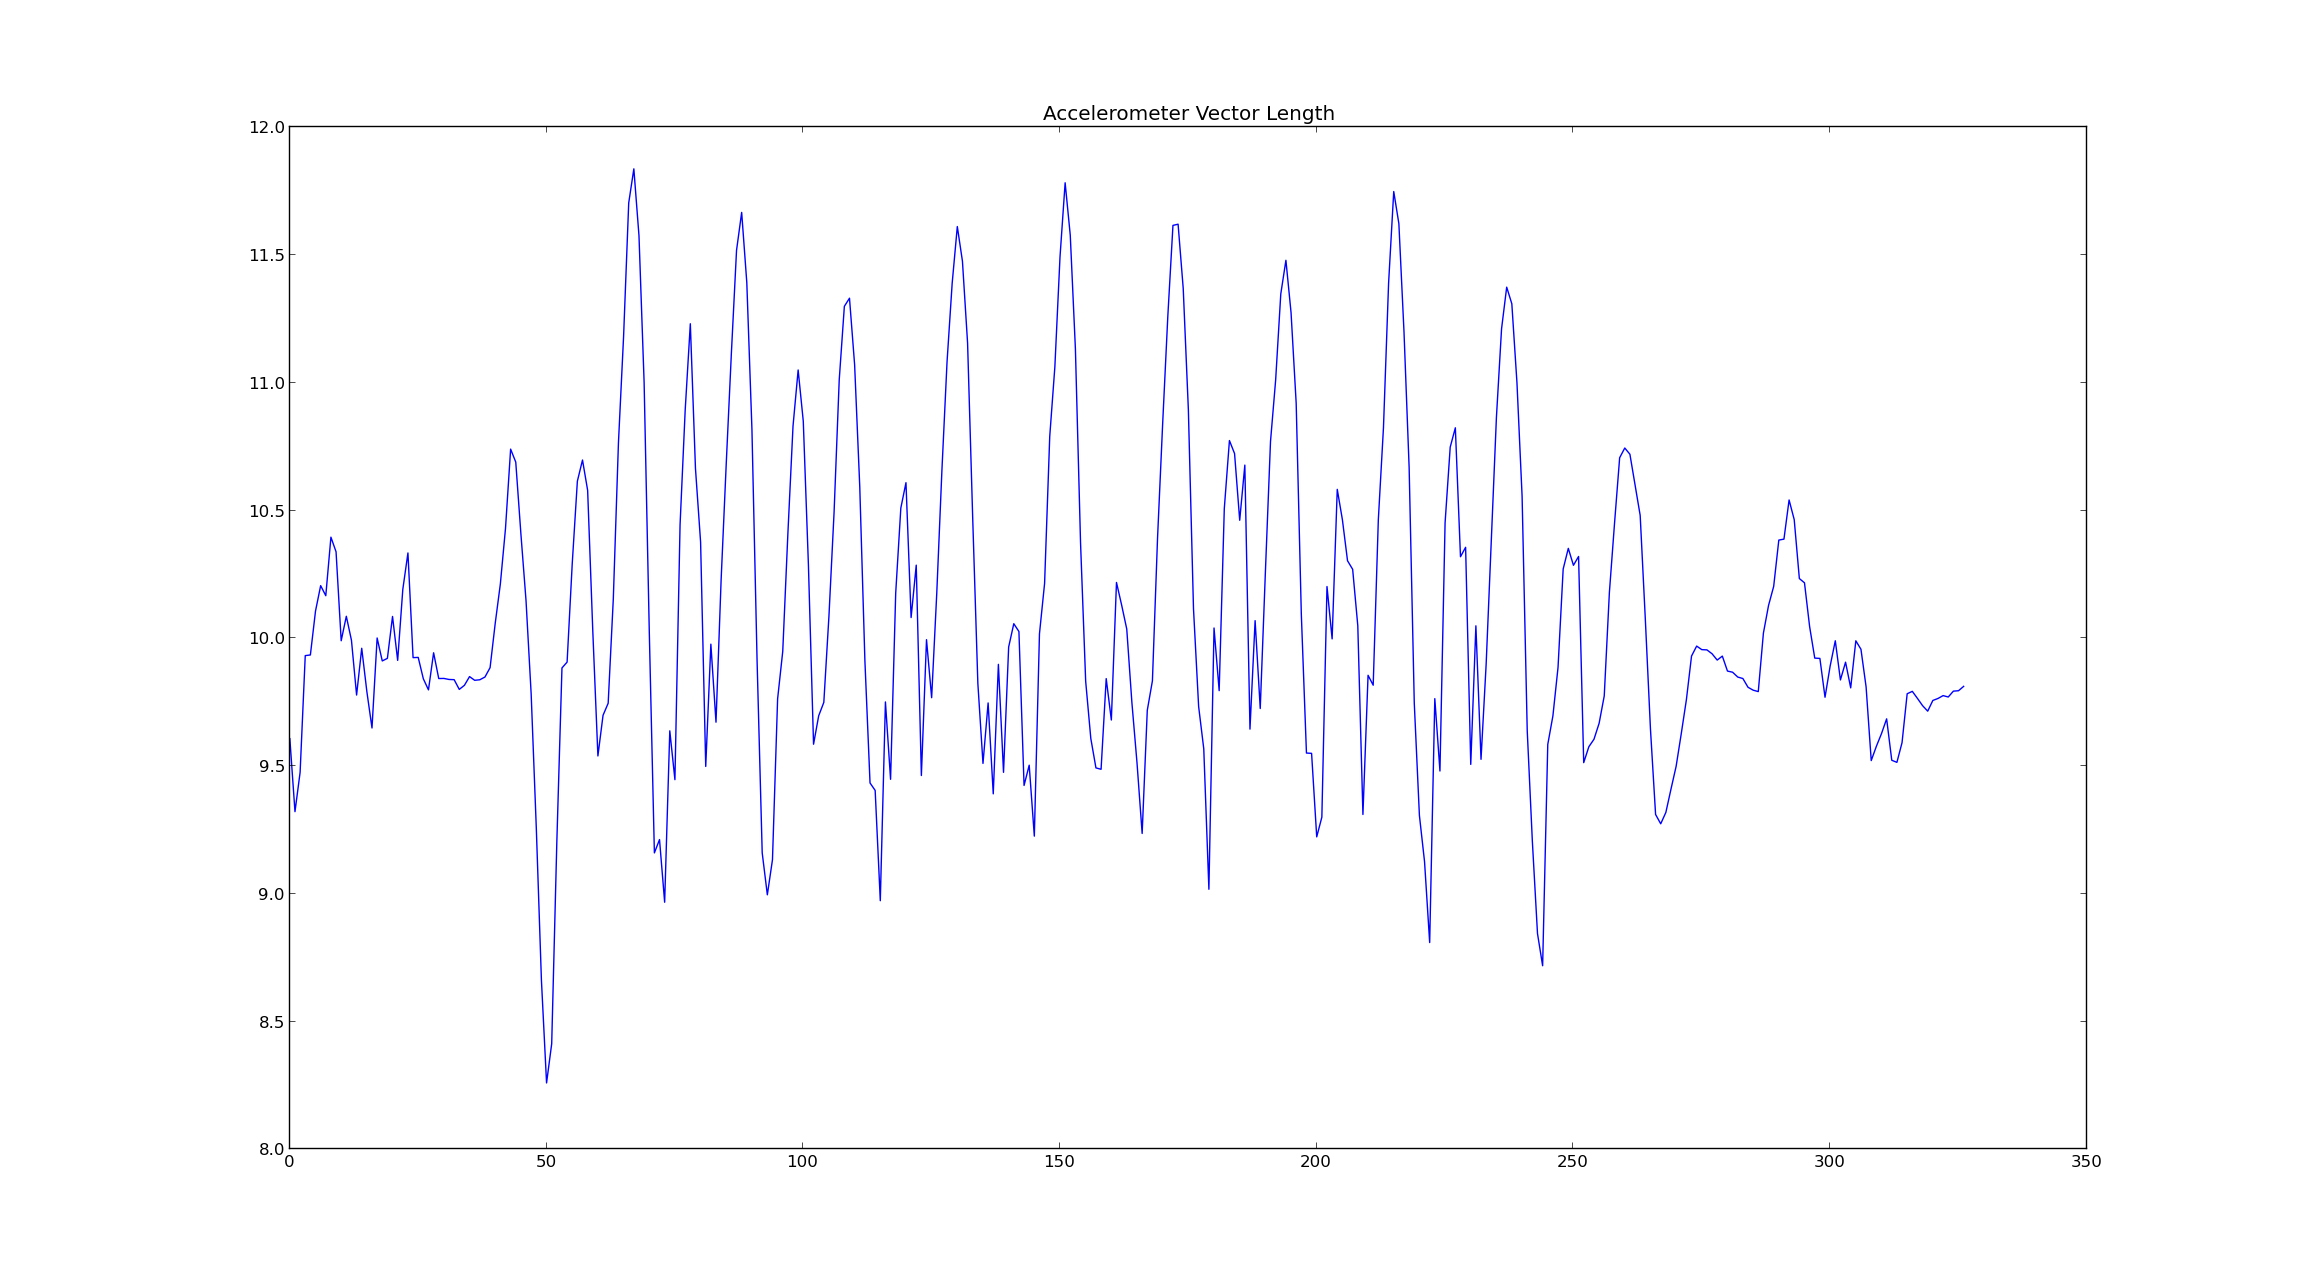
\includegraphics[width=1.45\textwidth , angle=0]{Res/FilipWalks}
}
}

\caption{A normal pattern of walking: Notice the alternating peak height in the middle.}
\label{fig:FilipWalks}
\end{figure}